\chapter{METHODOLOGY}

\begin{figure}[htb]
    \centering
    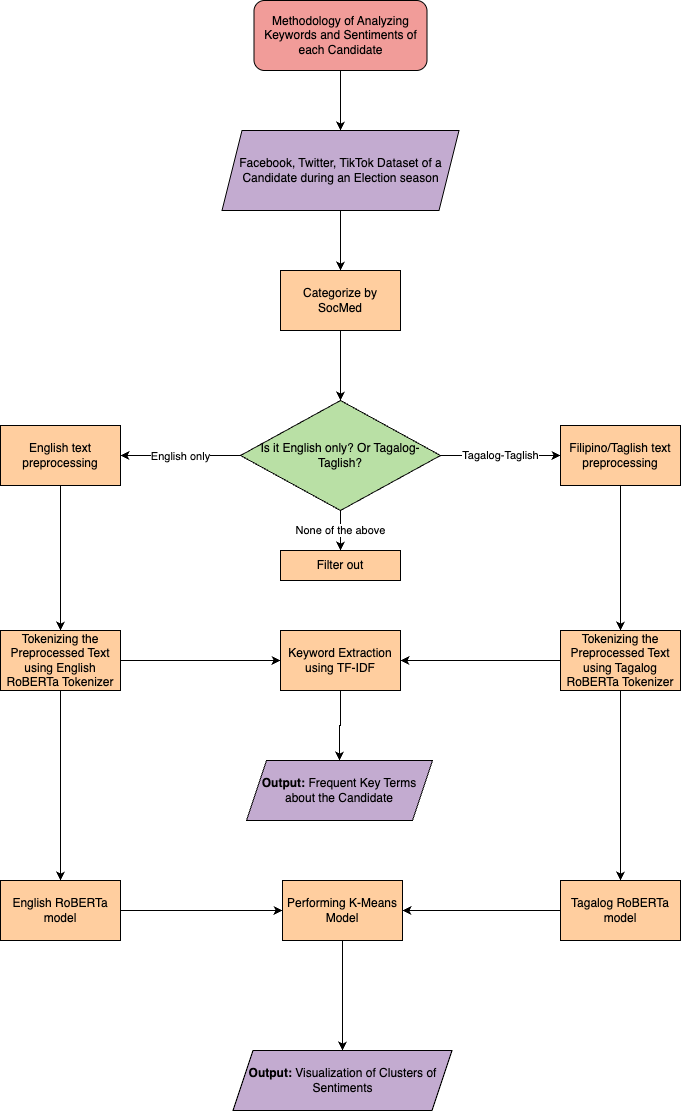
\includegraphics[width=0.82\textwidth]{Figures/methodology_flowchart.png}
    \caption{Research Methodology}
    \label{fig:Methodology}
\end{figure}

\section{Data Collection}
The collection of datasets will happen through the official Application Program Interfaces (APIs) of Twitter, Facebook, and TikTok. If the said APIs are unavailable or country-restricted, open-source tools will be used to collect posts and comments. Due to the unique nature of TikTok, which consists of either images or videos, it will just consist of captions of the video and comments. 

The dates of the posts and comments in the data will be as follows, starting from the day one of the candidates announced their nomination up to two days before the election day:

\begin{table}[!h]
    \centering
    \begin{tabular}{ |m{8em}|m{10em}|m{7em}| } 
        \hline
        Presidential Election years & Intention to Run Announcement &  End Date \\
        \hline\hline
        \multirow{2}{8em}{2016} & Duterte and Cayetano: November 21, 2015 & \multirow{2}{7em}{May 7, 2016} \\
        & Roxas and Poe: July 31, 2015 & \\ 
        \hline
        \multirow{2}{8em}{2022}& Marcos and Duterte: October 5, 2021 & \multirow{2}{7em}{May 7, 2022} \\
        & Robredo and Pangilinan: October 7, 2021 & \\
        \hline
    \end{tabular}
    \caption{Table for Philippine Dataset Ranges}
\end{table}

\begin{table}[!h]
    \centering
    \begin{tabular}{ |m{8em}| m{10em}|m{7em}| } 
        \hline
        Presidential Election Year & Intention to Run Announcement & End Date \\
        \hline\hline
        \multirow{2}{8em}{2020} & Biden and Harris: April 25, 2019 & \multirow{2}{7em}{November 6, 2020} \\
        & Trump and Pence: January 21, 2017 & \\ 
        \hline
        \multirow{2}{8em}{2024}& Trump and Vance: November 15, 2022 & \multirow{2}{7em}{November 6, 2024} \\
        & Harris and Walz: July 21, 2024 & \\
        \hline
    \end{tabular}
    \caption{Table for United States Dataset Ranges}
\end{table}

\section{Data Preprocessing}
Posts and comments will undergo preprocessing before feeding the data into the RoBERTa model. Since RoBERTa recognizes the stop words such as “the,” “a,” “is”, etc., it will not be removed during this process. The following steps to preprocess the text will be as follows:

\begin{enumerate}
    \item Removing punctuation marks that have no significance for sentiment analysis.
    \item Replacing emojis with special tags.
    \item Lowercasing the text.
    \item Handling links and email addresses by replacing them with a placeholder.
    \item Removing whitespaces and replacing multiple spaces with a single space.
    \item Adding paddings to equalize the length of sentences.
\end{enumerate}

\section{Text Classification}
After the preprocessing, they will be fed into the following models: the RoBERTa model for contextualized embedding and the TF-IDF model for determining frequent keywords. Since the standard RoBERTa model primarily uses an English dataset for pretraining, to handle Tagalog and Taglish language texts, the researchers will use the Tagalog RoBERTa model created by \textsc{DOST ASTI} \cite{MTHD_RoBERTa-model}. After the formulation of embeddings, they will be analyzed using the Classifier Pipeline function from the Transformers library, whose output will be used for clustering sentiments.